% ===========================================背景

\subsection{背景}
如前所述,在传统媒介向新媒体转换、融合的阶段中,现存两种实现方式,其一是以数字媒体为主的网络博客,而另一类则是以传统纸媒为主的数字报格式,本系统旨在为后者解决其Web化的工业化难题。

\paragraph{问题描述}

目前大多数数字报的Web化形式都仅停留在了形上,并未真正地融入了Internet元素。

那么什么是Internet,什么又是Web呢,简单地说,就是链接,两者都是增加了链接的数量与质量。例如谷歌、百度,是增进了网民获取所需的链接,而社交网络则是增进了人与人之间的链接,无论是何种形态的Web应用都是以人为出发点,去增进两种事物之间链接的应用程序。

而如今的数字报,从链接上仅仅是增加了一个从头版到文章的链接,但缺少了一个重要的因素,这样的链接并未从人、从用户的角度去考虑,无论是从浏览体验,还是其网络属性来说,都仅仅是将报纸铺在电子显示屏而已。

\noindent
那么真正的Web化是怎样的呢?可以分别从三个方面来逐一体现:
\begin{description}
	\item[分众] 细分用户群,对不同的用户群实现不同的运营策略,要做到这点,需要对用户数据进行收集、建模,为后两方面的实现提供基础数据模型。
	\item[精准] 精准是建立在分众之上,没有很好地细分用户,就没办法精准地了解到特定用户模型的刚性需求。
	\item[互动] 你的用户在使用产品时,需要一个快速、实时的平台与你进行交流,共同改进产品,而这种交流可以是显式的自然语言,同样也可以是其他形式来实现。
\end{description}

\noindent
本章节将会围绕这三个需求,慢慢向你揭开Web化报刊的神秘面纱。

\indent
但对于传统报社,因接不暇地业务需求遽增,同时又要分心涉足互联网,无疑是在蚕食其有限的战斗能力,此时该系统就应运而生,论文最后所实现的这一Web应用即是一个针对广大传统报社的SaaS(Software as a Service)云服务。

\indent
利用这一服务,注册的报社可以轻松地利用已有的资源,生成电子期刊,并获取在线订阅用户,作为一个纯粹的内容提供商(CP, Content Provider)的同时,我们还为报社提供其电子产品的用户数据,方便其针对数字用户制定相应的商业策略。

% ==========需求及系统功能分析===============================================

\subsection{需求及系统功能分析}
\subsubsection{目标用户}
该服务即一综合服务性平台,既拥有上节中说的企业级用户,同时作为一个报刊阅读平台,也拥有着以阅读为目标的个人用户。前者消费流量,而后者提供流量,从而构成了一个良性的生态循环。

\subsubsection{需求分析}
\paragraph{企业级用户}
这类用户的需求相对比较复杂,他们需要的是一个集数字报刊发布软件、数据统计平台为一体的云服务,我们除了提供此类服务之外,还应该尽量地简化他们发布数字报刊的时间成本,提供阅读质量。

\paragraph{个人用户}
这是一类需求相对简单的用户群,它们使用我们服务的理由就是以快速获取信息为主。因此我们需要提供一个各终端平台都无障碍的阅读平台,同时尽力地提高其阅读体验。

\subsubsection{功能分析}
\paragraph{数字报刊发布}
从企业级用户的根本需求出发,以节省其时间代价为根本,极力地简化其发布流程,用户在成功创建一类报刊后,在发布期刊时,仅仅需要上传一份PDF格式文件,我们的服务中心会提用户分析数据,提供适配所有终端的阅读页面。

\paragraph{数字报阅读平台}
从个人用户的根本需求出发,为他们提供一个易于阅读,易于分享的阅读平台。

\paragraph{数据统计平台}
同样为企业级用户量身定做,基于数据可视化技术为企业级用户快速、便捷地筛选出自己想要的信息。

\subsubsection{性能需求}
\begin{description}
	\item[高并发] 互联网应用与生俱来的高并发性要求无疑是对程序设计的一大挑战,因此整个系统需要低成本地解决高并发的问题。
	\item[数据安全] 系统应当保证用户能正常、稳定、安全地使用服务。
\end{description}

\subsection{小结}
根据以上需求分析,可以将系统划分为3个子模块,分为:用户/组管理、报刊发布与管理平台、阅读平台,如图1(Figure 1)。
\par~

\begin{figure}[h]
\begin{displaymath}
	\xymatrix{
	  			 && User/Group Management \\
	  System \ar[ur] \ar[r] \ar[dr] && Publication Platform \\
	  			 && Online Reader }
\end{displaymath}
\caption{系统模块分支}
\end{figure}

用户/组管理包括用户认证、用户分组两个功能项目。一是用以保证系统进入以及操作的安全性,二是用以差异化用户,分别针对企业级用户与个人用户,设置相应的操作权限。相对应的:企业级用户有权使用报刊发布管理平台的资源,对其发布的报刊进行发布、添加、删除、修改等管理,而个人用户作为流量提供者,仅仅能使用阅读平台,来满足自己的阅读需求,同时贡献流量。
\par

报刊发布与管理平台包括较为复杂,首先需要详细说明一下报刊与用户之间的关系。 \clearpage

\begin{figure}[t]
	\centering
		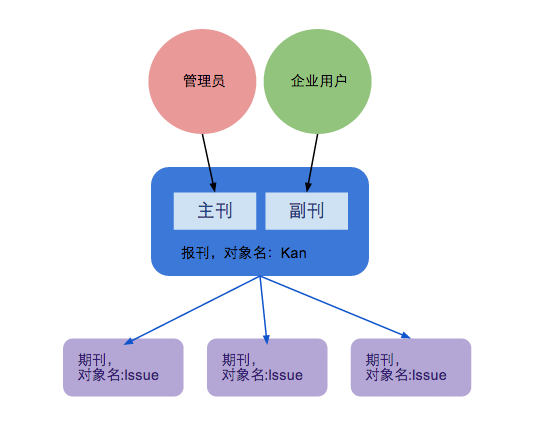
\includegraphics[width=0.8\textwidth]{./images/chap1-1.png}
	\caption{报刊/用户关系图}
\end{figure}

\noindent
对象Kan包含如下属性(Property):
\begin{description}
	\item[name] 报刊名字
	\item[user] 创建该报刊的企业或高级用户
	\item[group] 该报刊所属的分类,如:综合、科技等
	\item[tags] 创刊人为报刊添加的标签,用于更多元化的搜索
	\item[cover] 报刊的封面图片
	\item[description] 创刊人对该报刊的描述
\end{description}
\par~

\noindent
对象Issue包含如下属性(Property)
\begin{description}
	\item[title] 期刊的标题
	\item[date]  期刊发布时间
	\item[content] 期刊的内容
	\item[kan] 所属的报刊
\end{description}
\par~

\clearpage






